\chapter{Confidence Intervals}

The reason of using an interval estimator $[L(\mathbf{X}), U(\mathbf{X})]$ 
instead of a point estimator $\widehat{\theta}$ is that the interval estimator 
can have some level of confidence that the unknown parameter $\theta$ lies within the interval. 
The certainty of this guarantee is qualified by the following definitions.

\begin{definition}[Interval Estimator]
    Let $\mathbf{X} = (X_1, X_2, \ldots, X_n)$ be a random sample of size $n$ from a population with
    density function $f(x | \theta)$, where $\theta \in \Theta$ is an unknown parameter. The 
    \textbf{interval estimator} is a pair of statistics $[L(\mathbf{X}), U(\mathbf{X})]$ such that $L(\mathbf{X}) < U(\mathbf{X})$ for all possible samples $\mathbf{X}$.
\end{definition}

Another well known method for constructing confidence 
sets is that using the pivotal quantities.

\section{Pivotal Quantities}

\begin{definition}[Pivotal Quantity]
    A function $Q(X, \theta)$ is called a pivotal quantity (or pivot) 
    if and only if the distribution of $Q(X, \theta)$ does not depend on any unknown parameter $\theta$.
\end{definition}
\begin{remark}
    A pivot is not a statistic, although its distribution is known. 
\end{remark}

With a pivot $Q(\mathbf{X}, \theta)$, a confidence set on level $1 - \alpha$ for any $\alpha \in (0,1)$, can be obtained 
by finding a Borel set $\mathcal{A} = [c_1, c_2]$ such that $\mathbb{P}[Q(\mathbf{X}, \theta) \in \mathcal{A}] \geq 1 - \alpha$.
Then the set 
\begin{equation}
    C(\mathbf{X}) = \{ \theta \in \Theta \mid Q(\mathbf{X}, \theta) \in \mathcal{A} \}
\end{equation}
is a confidence set on level $1 - \alpha$ since
\begin{equation}
    \inf_{\theta \in \Theta} \mathbb{P}_\theta(Q(\mathbf{X}, \theta) \in \mathcal{A}) = \mathbb{P}[Q(\mathbf{X}, \theta) \in \mathcal{A}] \geq 1 - \alpha.
\end{equation}
If $Q(\mathbf{X}, \theta)$ has a continuous cdf, then we can choose $c_1$ and $c_2$ such that 
$C(x)$ has exact coverage probability $1 - \alpha$.

\begin{definition}[Location-Scale Family]
    Let $g : \mathbb{R} \to \mathbb{R}$ be a probability density function. Then for
    any $\mu$ and any $\sigma > 0$, the family of functions
    \begin{equation}
        \mathcal{F} = \left\{ f(x; \mu, \sigma) = \frac{1}{\sigma} g\left(\frac{x - \mu}{\sigma}\right) \mid \mu \in (-\infty, \infty), \sigma \in (0, \infty) \right\}
    \end{equation}
    is called the \textit{location-scale family} with standard probability density $f(x; \theta)$.
    The parameter $\mu$ is called the \textit{location parameter} and the parameter $\sigma$ is
    called the \textit{scale parameter}. If $\sigma = 1$, then $\mathcal{F}$ is called the \textit{location family}. If
    $\mu = 0$, then $\mathcal{F}$ is called the \textit{scale family}.
\end{definition}

It should be noted that each member $f(x; \mu, \sigma)$ of the location-scale
family is a probability density function. If we take $g(x) = \frac{1}{\sqrt{2\pi}} e^{-\frac{1}{2}x^2}$, then
the normal density function
\begin{equation*}
    f(x| \mu, \sigma) = \frac{1}{\sigma} g\left(\frac{x - \mu}{\sigma}\right) = \frac{1}{\sqrt{2\pi\sigma^2}} e^{-\frac{1}{2}\left(\frac{x-\mu}{\sigma}\right)^2}, \quad -\infty < x < \infty
\end{equation*}
belongs to the location-scale family. The density function
\begin{equation}
    f(x | \theta) = \begin{cases}
        \frac{1}{\theta} e^{-\frac{x}{\theta}} & \text{if } 0 < x < \infty \\
        0 & \text{otherwise,}
    \end{cases}
\end{equation}
belongs to the scale family. However, the density function
\begin{equation}
    f(x | \theta) = \begin{cases}
        \theta x^{\theta - 1} & \text{if } 0 < x < 1 \\
        0 & \text{otherwise,}
    \end{cases}
\end{equation}
does not belong to the location-scale family.

\begin{table}[h!]
\centering
\renewcommand{\arraystretch}{1.2}
\begin{tabularx}{0.45\paperwidth}{p{2.5cm} p{2.5cm} p{3cm}}
    \toprule
    Form of pdf & Type of pdf & Pivots \\[0.6em]
    \midrule
    $f(x - \mu)$ & Location & $\ols{X} - \mu$\\[0.6em]
    $\mfrac{1}{\sigma} f(\mfrac{1}{\sigma})$ & Scale & $\mfrac{\ols{X}}{\sigma}, \mfrac{S^2}{\sigma^2}, \mfrac{X_{(n)}}{\sigma}$\\[0.6em]
    $\mfrac{1}{\sigma} f(\mfrac{x - \mu}{\sigma})$ & Location-scale & $\mfrac{\ols{X} - \mu}{S}, \mfrac{S^2}{\sigma^2}$\\[0.6em]
    \bottomrule
\end{tabularx}
\caption{The location and scale families and some common pivots. Here, $\ols{X}$ is the sample mean, $S^2$ is the sample variance, and $X_{(n)}$ is the maximum order statistic.}
\end{table}

\section{Confidence Interval for Population Mean}

At the outset, we use the pivotal quantity method to construct a confidence interval for the mean of a normal population. 
First we assume that the population is normal and the population variance is known, but the variance is unknown. Next, we
 construct the confidence interval for the mean of a population with continuous,
 symmetric and unimodal probability distribution by applying the central
 limit theorem.

We know that $\widehat{\mu} = \ols{X}$. Because each $X_i$ is identically distributed as $N(\mu, \sigma^2)$,
the distribution of the sample mean $\ols{X}$ is given by

\[
\ols{X} \sim N\left(\mu, \frac{\sigma^2}{n}\right).
\]

It is easy to verify that the distribution of the estimator $\widehat{\mu}$ is not independent of the parameter $\mu$. 
If we standardize $\widehat{\mu}$, we have

\[
Z = \frac{\ols{X} - \mu}{\sigma / \sqrt{n}} \sim N(0, 1).
\]

However, the distribution of the standardized variable $Z$ is independent of the parameter $\mu$. Thus, $Z$ is a pivotal quantity
since it is a function of the sample $X_1, X_2, \ldots, X_n$ and parameter $\mu$. Using this 
standardized variable as the pivotal quantity, we can construct a confidence interval for the population mean $\mu$
as follows:
\begin{align*}
    1 - \alpha &= \uprob[\mu \sim \ols{X}]{-z_{\alpha / 2} \leq Z \leq z_{\alpha/2} }\\
    &= \uprob[\mu \sim \ols{X}]{ -z_{\alpha / 2} \leq \frac{\ols{x} - \mu}{\sigma / \sqrt{n}} \leq z_{\alpha/2} }\\
    &= \uprob[\mu \sim \ols{X}]{ \ols{x} - z_{\alpha / 2} \frac{\sigma}{\sqrt{n}} \leq \mu \leq \ols{x} + z_{\alpha/2} \frac{\sigma}{\sqrt{n}} }.
\end{align*}

Hence, the $(1-\alpha)100\%$ confidence interval for $\mu$ when the population $X$ is normal 
and known variance $\sigma^2$ is given by

\begin{equation}
    \ols{x} \pm z_{\alpha / 2} \frac{\sigma}{\sqrt{n}}
\end{equation}

To interpret the confidence interval of $\mu$, we say that 
if you repeating the same experiment process many times, and
generate a confidence intervals using the same method. Then approximately $(1-\alpha)100\%$ of the intervals will contain the true value of $\mu$.
\begin{figure}[!ht]
    \centering
    \makebox[\textwidth]{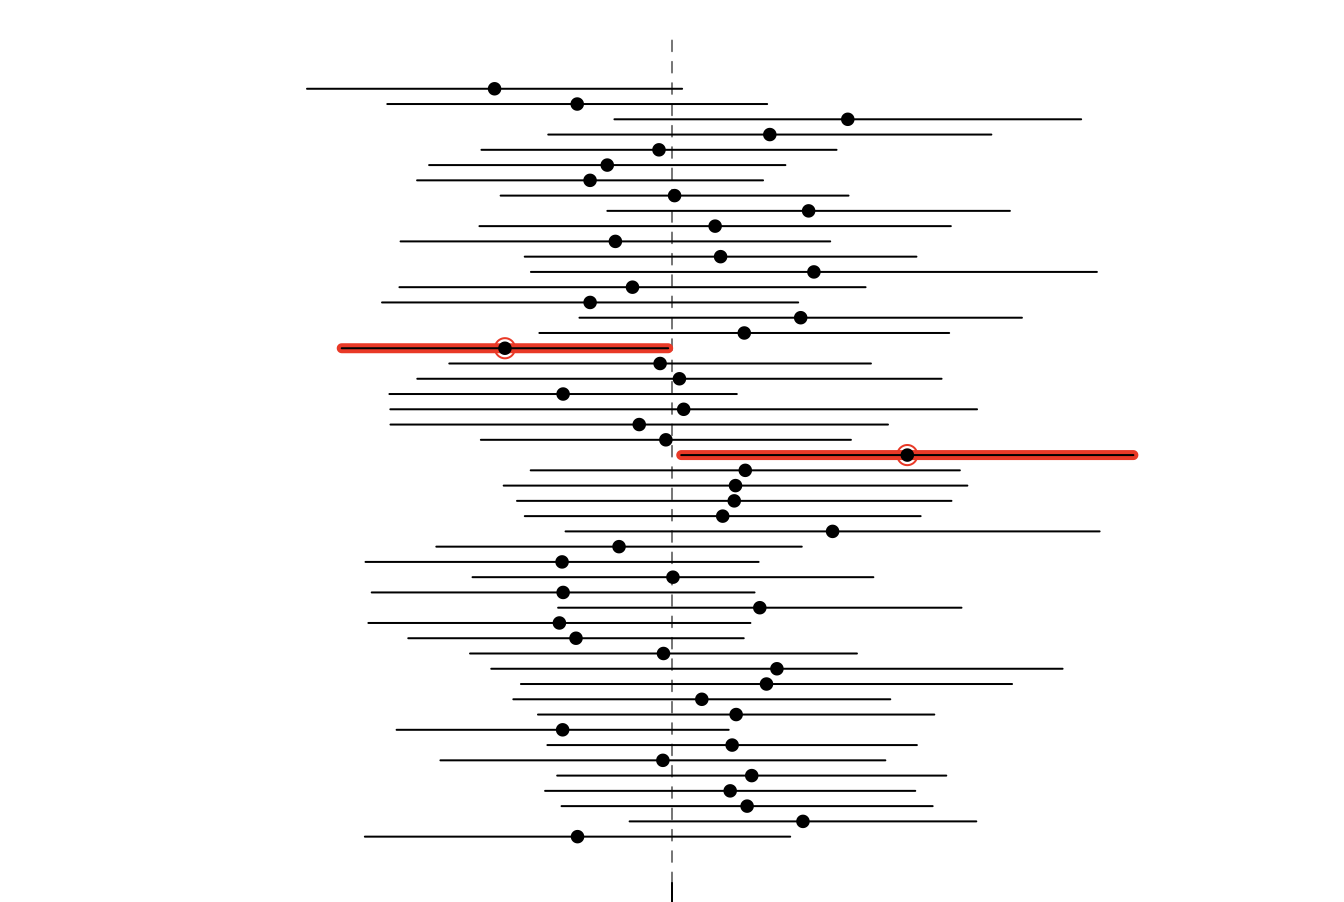
\includegraphics[width=0.7\paperwidth]{./images/confidence_int.png}}
    \caption{This is a simulation of the confidence interval for the population mean. We generate 50 samples of size 30 from a normal population with mean 50 and standard deviation 15.
    The red horizontal line indicates the true mean of the population do not include the true population mean. Observe that 
    48 out of 50, of the intervals contain the true mean. Thus, the coverage probability is approximately 96\%.}
\end{figure}

\begin{example}
    Let $X_1, X_2, \ldots, X_{11}$ be a random sample from a normal population with unknown mean $\mu$ and variance $\sigma^2 = 9.9$.
    Given that $\sum_{i=1}^{11} x_i = 132$. Find a 95\% confidence interval for $\mu$.
\end{example}
\begin{solution}
    From the information above, the sample mean is 
    \[
    \ols{x} = \frac{\sum_{i=1}^{11} x_i}{11} = \frac{132}{11} = 12.
    \]
    Furthermore, since $\mu$ is unknown, we use $\widehat{\mu} = \ols{x} = 12$. Since each $X_i \sim N(\mu, \sigma^2=9.9)$, 
    the confidence interval for $\mu$ at 95\% confidence level is
    \begin{align*}
        \ols{x} \pm z_{\alpha / 2} \frac{\sigma}{\sqrt{n}} &= 12 \pm z_{\mfrac{0.05}{2}} \sqrt{\frac{9.9}{11}} \\
        &= 12 \pm 1.96 \sqrt{0.9}.
    \end{align*}
    That is
    \[
        [10.141, 13.859].
    \]
\end{solution}

\section{Confidence interval for unknown variance}

Consider a random sample $X_1, X_2, \ldots, X_n$ from a normal population with mean $\mu$ and variance $\sigma^2$. 
When both $\mu$ and $\sigma^2$ are unknown, we can use the sample variance $S^2$ to estimate the population variance $\sigma^2$.
We know that 
\[
\frac{(n-1)S^2}{\sigma^2} \sim \chi^2_{n-1} \implies \frac{\sum^n_{i=1} (X_i - \ols{X})^2}{\sigma^2} \sim \chi^2_{n-1}. 
\]
We take $Q(X_1, \ldots, X_n, \sigma^2) = \displaystyle \frac{\sum^n_{i=1} (X_i - \ols{X})^2}{\sigma^2}$ as a pivotal quantity to construct
the confidence interval for $\sigma^2$. Hence, we have 
\begin{align*}
    1 - \alpha &= \uprob[\sigma^2]{\frac{1}{\chi^2_{n-1, \alpha / 2}} \leq Q \leq \frac{1}{\chi^2_{n-1,\> 1 - \mfrac{\alpha}{2} }} }\\
    &= \uprob[\sigma^2]{ \frac{1}{\chi^2_{n-1, \alpha / 2}} \leq \frac{\sum^n_{i=1} (X_i - \ols{X})^2}{\sigma^2} \leq \frac{1}{\chi^2_{n-1,\> 1 - \mfrac{\alpha}{2} }} }\\
    &= \uprob[\sigma^2]{ \frac{\sum^n_{i=1} (X_i - \ols{X})^2}{\chi^2_{n-1,\> 1 - \mfrac{\alpha}{2}}} \leq \sigma^2 \leq \frac{\sum^n_{i=1} (X_i - \ols{X})^2}{\chi^2_{n-1,\> \mfrac{\alpha}{2} }} }
\end{align*}

Hence, the $100(1 - \alpha)\%$ confidence interval for $\sigma^2$ when the population mean is unknown is given by 
\[
\left[ \frac{(n-1)S^2}{\chi^2_{n-1,\> 1 - \mfrac{\alpha}{2}}} ,\quad \frac{(n-1)S^2}{\chi^2_{n-1,\> \mfrac{\alpha}{2}}} \right].
\]